\documentclass[12pt, a5paper]{bxjsbook}
\usepackage{koseneducators}
\usepackage{zxjatype}
\usepackage[ipa]{zxjafont}
\title{Chapter1}
\date{\today}
\begin{document}
\tableofcontents
\chapter{Sympyとは何か?}
近頃、空前の機械学習ブームの到来などがキッカケとなって、基礎/応用数学を学ぶ人や、 {\bf Python}というプログラミング言語を使って計算、データ分析等を行う人が世の中で飛躍的に増加しました。
\subsection{Pythonとは}
Python\footnote{「ぱいそん」と読みます。}を使うと、従来のプログラミング言語では非常に面倒、あるいは難解だったような複雑な処理や計算が、とても簡単に直感的に行えます。筆者は3つくらいのプログラミング言語を使えますが、Pythonの{\bf 「直感性」「面倒なことは考えなくて良いシンプルさ」}はまさに特筆すべき利点と言えるでしょう。
\subsection{数学を学ぶハードル(1) 〜「突然の機械学習ブーム」の観点で〜}
そして、Python需要と同時に高まったのが{\bf 「数学需要」}です。数学は、昔々から学校教育の中でずーっと扱われ続けていますが、「受験勉強のために仕方なく勉強するもの」というイメージが強く根付いていることが事実でした。しかし、近頃は突然の機械学習ブームを皮切りに「数学」という学問の重要性を誰もが認識するようになりました。だって、これだけ毎日毎日話題になっている{\bf 「AI(人工知能)」}を司る「機械学習」のアルゴリズムは、ほぼ完全に数学によって記述されているのですから。「AI」の原動力となる仕組みは、もっぱら数学だと言っても過言ではありません。

しかしながら、筆者がこの「AIブーム」の最中、誰もが「数学」を学ぼうと試みる様子を見ながら強く感じたことは、{\bf 「やはり数学の学習は鬼門なのだな」}ということだったりします。というのも、無理はないのです。高校、あるいは大学を卒業してITのお仕事をはじめて、結構な間数学とは遠い世界でお仕事をしていたところ、突然訪れてしまったこの「AIブーム」の中で、世の中が「数学が重要だ!」「数学を勉強しないと!」なんてまたたく間に色めきだつのですから。戸惑うに決まっています。今まであんなに、「数学はお金にならない」「数学科は就職がないから工学部に進学したほうがいい」なんて、世間から完全に「食えない学問の代表格」扱いされまくっていたあの数学がですよ。

当然、数学なんてしばらく触っていない。そんな日々の中で、数学の知識もまるっと頭から抜けてしまった。でも、機械学習の本なんかを読んでみれば、「ここは活性化関数を微分して...」「ここでこのベクトルをこの行列で線形変換して...」「この分布の確率密度関数は...」なんて言葉が「知ってますでしょ?」みたいに列挙されています。あぁ、一体どうすればいいんだろう...なんて時代に生まれてしまったんだ...なんてことを感じている方も多いかもしれません。

ここで一言皆さんにお伝えしておきます。そんな悩みを抱えている方には、{\bf 「Sympy」\footnote{「しむぱい」と読みます。}を使うのがおすすめです}(詳しくはまた後で)。

\subsection{数学を学ぶハードル(2) 〜「学校での学び」の観点で〜}
中学校までの間に学ぶ「数学」と、高校で学ぶ「数学」、そして大学で学ぶ「数学」の間には、それぞれ結構な隔たりがあって、どれも独自の難しさと面白さを兼ね備えています。

その中でやはり最も皆さんにとって壁になりやすいのが、「式変形」\footnote{数式をイコールで結びながら、違う形に変形すること。または、それを繰り返すこと。}です。中学校くらいまでの数学であれば、そんなに難しい式変形に出会うこともありませんが、高校、大学へと進んで行くと、そこで現れるのはいくつにでも連なる式変形の嵐。例えば、高校数学で「基本」と言われる操作、「二次関数の平方完成」ひとつとっても、式変形を丁寧に追いかければ以下のようになります\footnote{本書では、数式変形の終わりを$\Box$記号で表します。}。
\begin{align*}
    y &= 2x^2 + 8x + 3\\
    &= 2(x^2+4x)+3\\
    &= 2(x^2+4x+4-4)+3\\
    &= 2(x^2+4x+4)-8+3\\
    &= 2(x+2)^2-5\ \ \Box
\end{align*}
この式変形を手計算でゴリゴリと進める間、だんだんと頭の中がぼんやりとした不安で埋め尽くされてきます。「これ、計算合ってるんだろうか...??」そんな中で、数学を学び続けることが徐々にしんどくなってきて、結局のところ、「あぁ、自分は数学には向いていないのかもしれない...」なんて、心がぽっきり折れてしまうなんてことも少なくありません。

ここで一言皆さんにお伝えしておきます。そんな悩みを抱えている方には、{\bf 「Sympy」を使うのがおすすめです}。
\section{Sympyとは?}
こんなふうに、「数学」を学ぶことは、(もちろんその向こう側に楽しさはあれど)なかなかにしんどい気持ちになる作業の連続だと感じてしまうことも少なくないものです。

こんな悩みと日々格闘されながら、それでも式変形とうんうん唸りながら向かい続ける方々を目の当たりにして、筆者もいろいろと考えました。{\bf どうにかして、この負担をうまく軽くする方法はないものだろうか?}ということを。そしてその結果、「現代人の超効率的数学勉強法」として、このやり方こそベストソリューションなのではないか!?という方法を見つけ出すに至りました。それが、
\begin{center}
{\bf 「面倒な式変形はSympyにある程度投げてしまう」}
\end{center}
というアプローチです。

{\bf Sympy}とは、プログラミング言語「Python」上で動く、式変形などの数学的操作を、秒速かつ正確に行ってくれるモジュール\footnote{モジュールとは、簡単にいうと「プログラミング言語を構成する便利機能の集まり」のようなもののことを指します。}のひとつです。Python上でSympyを動かしてしまうことによって、我々が「面倒」だと思う式変形を(ほぼ)全自動で行うことができ、さらに、機械学習の専門書や学校の問題集の式変形の行間を埋めることも非常に容易になります。

ここで一つ断っておきたいこととして、「手計算のやり方なんて知らなくても数学を学ぶのに問題はない」ということを主張しているわけではありません。ただ、「毎回毎回、同じような面倒な式変形を手ですべて行う」必要は、この現代そんなにないのかもしれませんし、あるいは、「自分の手計算が正しいのかどうか」を確かめる術というのは、意外とそんなになかったりもするものです。こういう「数学を学ぶ上でぶち当たる面倒な問題」を、Sympyは「最新技術」の力である程度解決してくれるのです。

しかも、Sympyを使うことはとても簡単です。面倒な環境構築等もほとんど必要ありませんし、使い方も極めて明快で、誰もが簡単に、このSympyの恩恵に預かることが出来ます。この「数学の重要性」が当たり前のように語られるになった世の中、こんなに便利なアプローチを使わない手はありません。
\section{Sympyでできること}
Sympyを使うと、以下のような数学的操作を簡単に行うことができます。ここでは詳細な説明を省き、簡単に実例を交えながらこれらの「便利機能」を俯瞰してみてみることにしましょう。もちろん、数学的な理論の説明はまだしていないわけですから、皆さんは「おぉー、なんか知らないけどめっちゃ便利そうだな」くらいの気持ちで眺めていただければ問題ありません。
\begin{itemize}
    \item 
    式の四則演算、展開、因数分解など、簡単な式の計算を行う。
    \item
    初等関数(多項式、指数関数、対数関数、三角関数など)を扱ったり、グラフを描画する。
    \item
    方程式を解く。
    \item
    微分、積分などの計算を行う。
    \item
    ベクトル、行列、行列式など、線形代数と呼ばれる分野の計算を行う。
    \item
    その他、複素数や組合せなどの計算を行う。
    \item
    機械学習で必要になるような式変形の数々を行う。
\end{itemize}
\subsection{簡単な式の計算}
\begin{framed}
\begin{exq}
次の式を因数分解せよ。
$$x^3+8x^2+3xy+24y$$
\end{exq}
\end{framed}
\begin{enumerate}[(i)]
    \item 
    {\bf 手計算による解法}
    
    次数が小さい$y$について、降べきの順に整理すると、
    \begin{align*}
        &3xy+24y+x^3+8x^2\\
        &= 3y(x+8)+x^2(x+8)
    \end{align*}
    共通因数$(x+8)$でくくると、
    $$(x+8)(x^2+3y)\ \ \Box$$
    \item
    
    {\bf Sympyによる解法}
    \begin{center}
    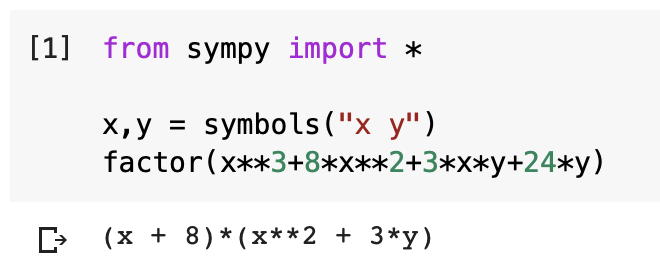
\includegraphics[scale=0.5]{fig1-2-1.png}
    \end{center}
\end{enumerate}
特筆すべき点は、{\bf 手計算による解法}では、「解法」を人間が頭で考えて、そのとおりの変形を行って答えにたどり着いているのに対し、{\bf Sympyによる解法}では、「$x,y$という文字を使いますよ」「この式を因数分解してください」と、「指示」を与えるだけで正しい答えが得られているところです。この2つの解法は、「人間がウンウン唸りながら考える」というプロセスの有無という意味で、天と地の差くらいの面倒さの違いがあります。
\subsection{初等関数を扱う}
\begin{framed}
\begin{exq}
次の関数$f(x)$のグラフを描画せよ。
$$f(x) = x^2e^{-x}$$
\end{exq}
\end{framed}
\begin{enumerate}[(i)]
    \item 
    {\bf 手計算による解法}
    
関数$f(x)$の1階導関数、2階導関数を計算し、関数の増減、凹凸を調べ、増減表を作成してそれをもとにグラフを描く。\\
    \item
    {\bf Sympyによる解法}
    \begin{center}
    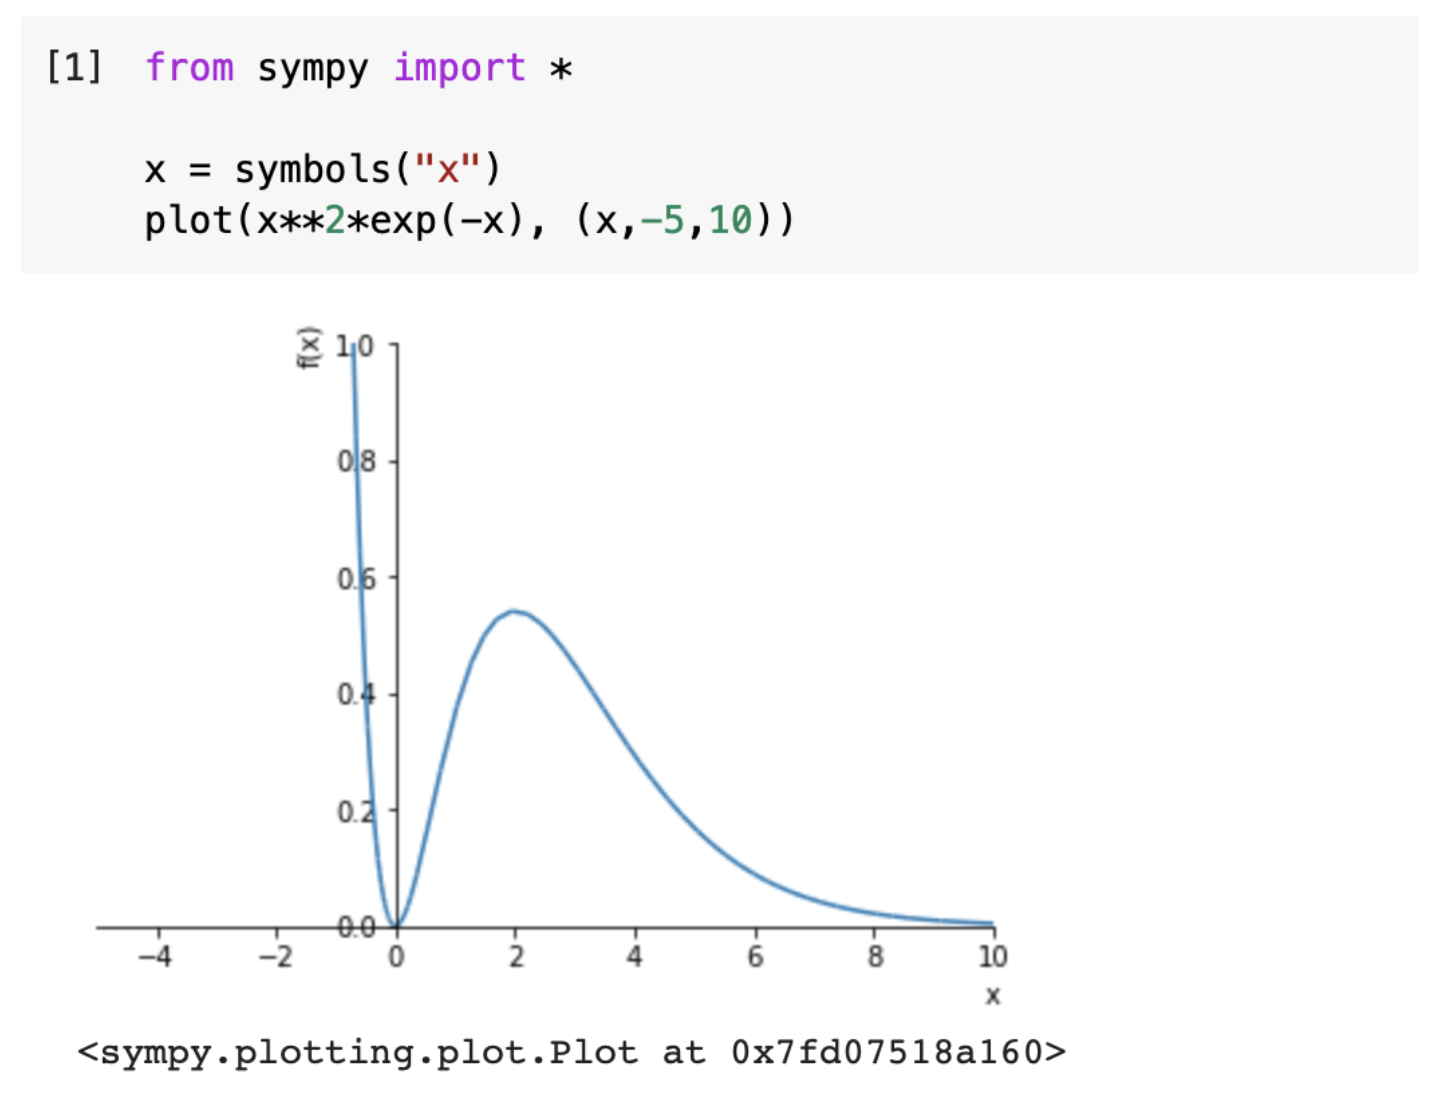
\includegraphics[scale=0.3]{fig1-2-2.png}
    \end{center}    
\end{enumerate}
この例でも、手計算による「増減表」を用いた方法だと、かなりの大きな手間がかかります。しかし、Sympyを用いた方法は、「$x$という文字を使いますよ」「この関数のグラフ描いてくださいね」と指示を与えるだけで、非常に正確なグラフを描いてくれています。

\subsection{方程式を解く}
\begin{framed}
\begin{exq}
次の方程式の解を求めよ。
$$3x^3+2x^2+x+10 = 0$$
\end{exq}
\end{framed}
\begin{enumerate}[(i)]
    \item 
    {\bf 手計算による解法}
    
多分これを手計算で解くには、以下の{\bf 3次方程式の解の公式}\footnote{フェラーリの公式、カルダノの公式などと呼ばれることもあります。長過ぎるのでかなり小さく記載しました。}を使うしかないでしょう(あるいは、センスのある人ならば{\bf 因数定理}で解くことも奇跡的にできるかもしれません)。
    \begin{center}
    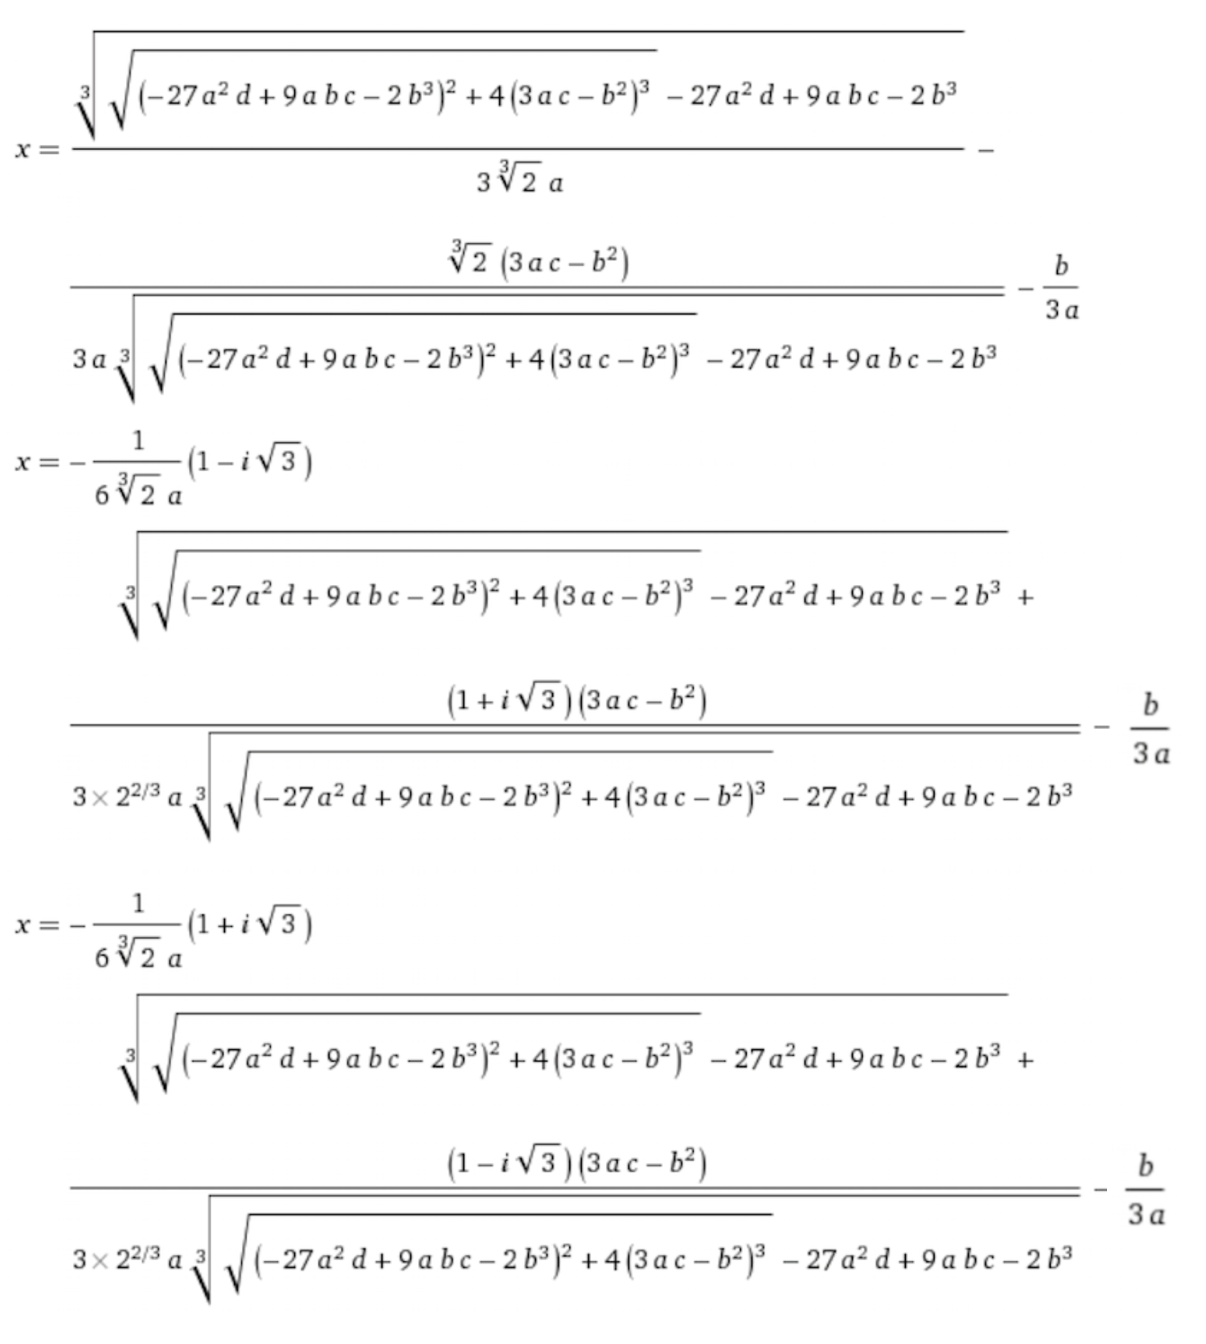
\includegraphics[scale=0.3]{fig1-2-4.png}
    \end{center}    

    \item
    {\bf Sympyによる解法}
    \begin{center}
    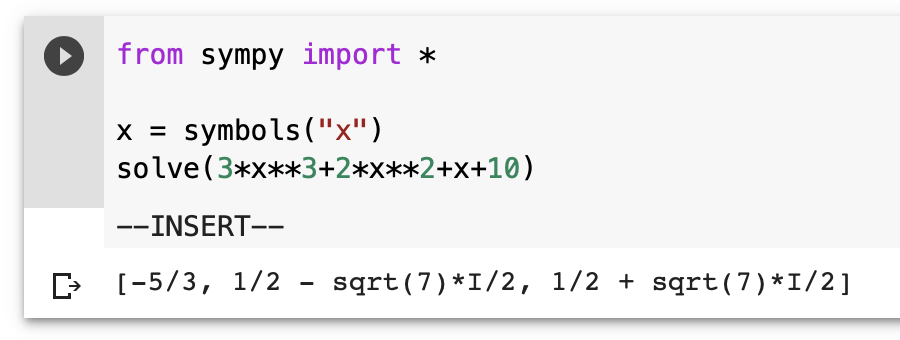
\includegraphics[scale=0.5]{fig1-2-3.png}
    \end{center}    
\end{enumerate}
あらあら、手計算ではまぁそう簡単には解けないだろうなという方程式でも、解が$x = -\frac53, \frac12 - \frac{\sqrt{7}}{2}i, \frac12 + \frac{\sqrt{7}}{2}i$であることが一瞬でわかってしまいました。
\subsection{微分や積分の計算}
\begin{framed}
\begin{exq}
次の関数$f(x)$を微分せよ。
$$f(x) = e^{ax}\sin{bx}$$
\end{exq}
\end{framed}
\begin{enumerate}[(i)]
    \item 
    {\bf 手計算による解法}

積の微分法則を用いて計算する。
\begin{align*}
    \frac{df}{dx} &= (e^{ax})'\sin{bx} + e^{ax}(\sin{bx})'\\
    &= ae^{ax}\sin{bx} + be^{ax}\cos{bx}
\end{align*}

    \item
    {\bf Sympyによる解法}
    \begin{center}
    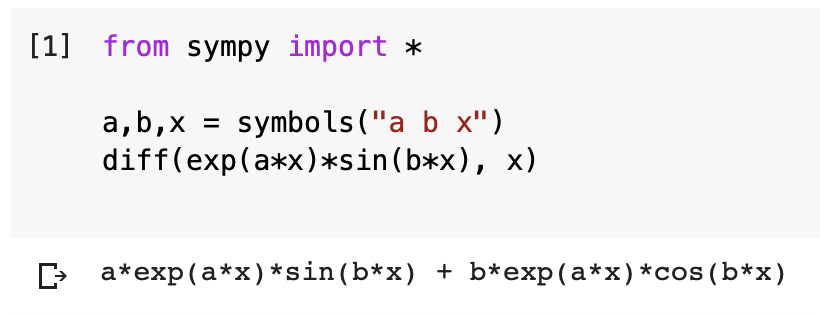
\includegraphics[scale=0.5]{fig1-2-5.png}
    \end{center}    
\end{enumerate}
微分の計算を行うには、関数の形に合わせた微分公式や微分公式を熟知した上で選択できなければなりません。それを「知らなくても良い」というわけでは決してありませんが、このくらいの微分計算なら、Sympyでやったほうが簡単で正確ですね。
\subsection{ベクトル、行列、行列式に関する計算}
\begin{framed}
\begin{exq}
次の行列$X$の逆行列を求めよ。ただし、$a$は定数である。
$$X=\begin{pmatrix}
1 & -a & 0\\
0 & 1 & -a\\
0 & 0 & 1
\end{pmatrix}$$
\end{exq}
\end{framed}
\begin{enumerate}[(i)]
    \item 
    {\bf 手計算による解法}

{\bf 3次逆行列の公式}、{\bf または掃き出し法(ガウスの消去法)}などを使って求めます(どちらも結構めんどくさいのでここに詳細を書く必要もないかと思います。気になる方は線形代数の教科書読んでみてください)。\\

    \item
    {\bf Sympyによる解法}
    \begin{center}
    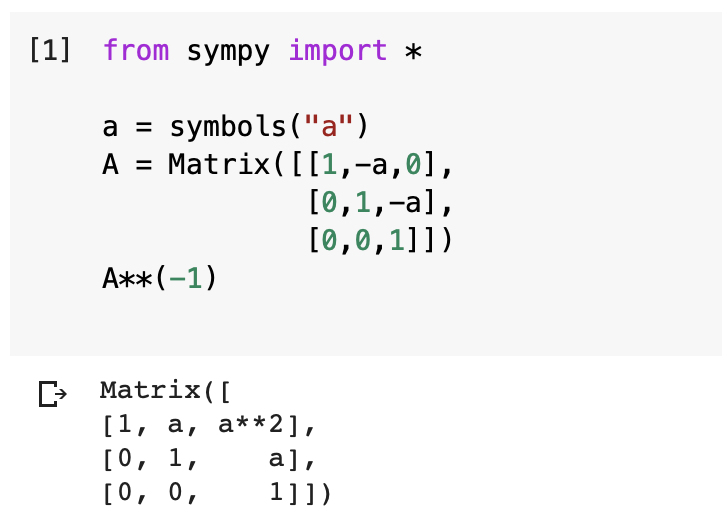
\includegraphics[scale=0.5]{fig1-2-6.png}
    \end{center}    
\end{enumerate}
この結果のすごいところは、$X$が文字($a$)が含まれる行列であるにも関わらず、何も言わずにさらっと逆行列を計算してくれているところです。このような「文字を含む式変形などの計算」のことを「代数的計算」と呼び、それに対して「数字だけの計算」を「数値的計算」と呼びます。プログラミング言語というのは、本来「数値的計算」は得意ですが、「代数的計算」は不得手なのです。しかし、Sympyはいとも簡単にこのくらいの計算は正確に行ってくれます。
\section{本書の目標 〜Pythonを超高性能電卓として使いこなせ!〜}
Sympyを使うと、様々な面倒な計算がいとも簡単に、しかも瞬速&正確に行なえることを何となく、感じて頂けましたか。Python上で使えるモジュール(ライブラリ)は何もSympyに限るわけではなく、他にも非常に優秀な機能をPython上でゴリゴリ動かし、人間の手助けをしてもらうことが十分に可能です。

しかし、このSympyというモジュールひとつだけをとっても、この威力は計り知れないと思っています。なんと言っても「代数的計算」を非常に気軽に行えること、そして、使い方がとても簡単で、それでいて高機能であることなど、利点を挙げれば正直キリがありません。他のモジュールなどは、非常に便利ではあるが、使用方法が難解、あるいは高度な計算に特化していて数学入門の段階では使いにくいなど、やや我々にとっては不都合な性質を持っていることも多いのです。

本書では、このSympyに焦点を絞って(他のモジュールは思い切って見なかったことにして)、様々な数学的操作がこのSympyで驚くほど自在に行えることを体感し、皆さんがPythonを「超高性能電卓」として使いこなし、数学の学習や実務での応用における非常に強力な武器として振りかざしていただける、という状態までたどり着くことを目標とします。

何度もいいますが、Sympyの使い方は驚くほど簡単です。そして強力です。そしてこのSympyを使いこなして習得する「数学の力」は、我々の業務や学習、さらには世界の見え方まで変えてしまう強大な力を秘めています。ぜひ、皆様と一緒にそこまでたどり着けたら、筆者としては光栄に思います。

それでは、早速本論を始めていきましょうか。Sympyの世界へようこそ!
\chapter{Pythonの基本の基本}
Sympyは、Python上で動くモジュールの一つです。すなわち、Python
の基本的な使い方を知らなければ、Sympyもあまり自由に使いこなすことができません。この章では、「全く何も分からない」状態から、Pythonの「基本の基本」を身につけることを目標にしましょう。
\section{Pythonの環境構築 〜Google Colaboratory〜}
まずは、お手元のPCでPythonが動作する環境を整えなければお話は始まりません。というわけで、早速環境構築を...という前に、少しだけお話を。

実はちょっと昔ですと、お手元のPCの中にPythonの環境を構築するために、なかなかに面倒な手順が必要でした。様々なアプリケーションをダウンロードして、これとこれとこれをインストールして、いざ動かしてみるとあれ?なんかエラーでうまく動かない...こんな格闘を繰り広げるのが、通過儀礼になっていた時代もあったのです。なんなら、Pythonを一度も触ることなく、この環境構築で挫折してしまう、なんて人も...。

でもこんな、最初の一歩で心が折れてしまうのってあまりにも悲しいじゃないですか。そんな悲痛な叫びを察知してくれたのか、現在はGoogleのサービス{\bf 「Google Colaboratory」}を用いると、ものの数分で環境構築が誰でも簡単に、完璧に終わってしまいます。本書ではこの「Google Colaboratory」を使って、さくっと環境構築を済ませてしまうことにしましょう。

\begin{enumerate}[手順1.]
    \item 
    {\bf Googleアカウントを取得する}
    
     まず、Googleアカウントを取得してください(この手順はここでは解説しませんが、やりかたが分からない方は検索すればすぐにわかります)。\\
     
    \item
    {\bf Google driveを開く}
    
     作ったGoogleアカウントにログインし、Google driveを開きます。 
    \begin{figure}[h]
     \centering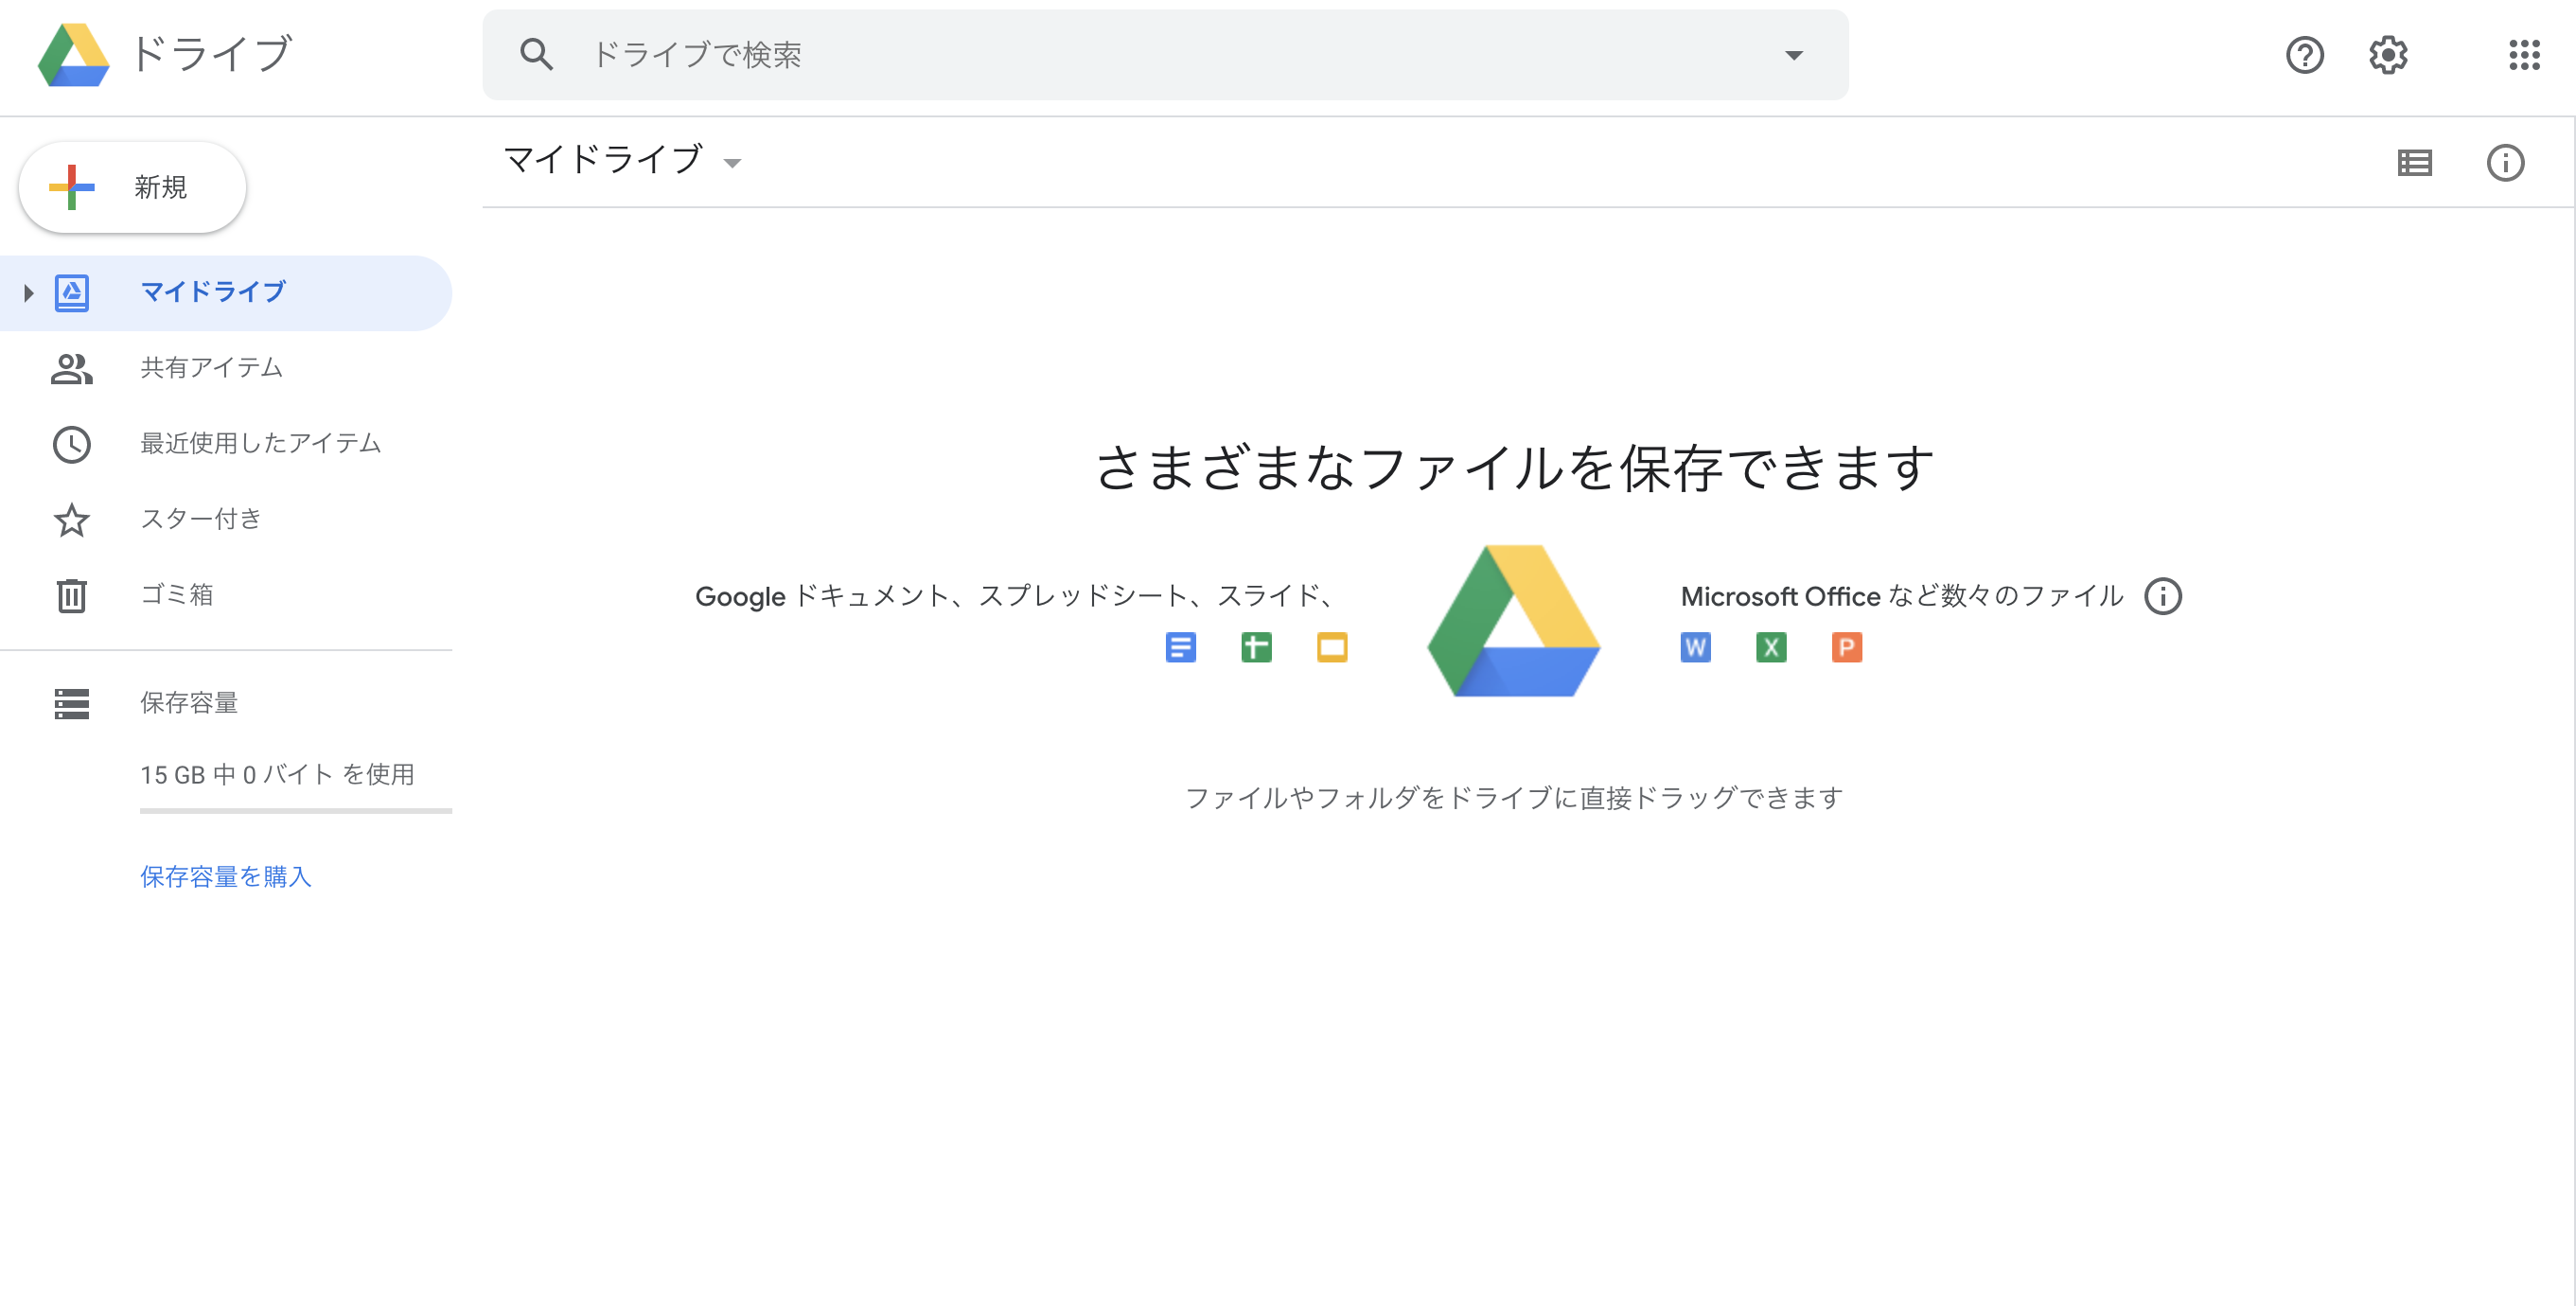
\includegraphics[scale = 0.15]{fig2-1-1.png}\caption{Google driveを最初に開くとこんな感じ(何もファイルは入っていない)。}
    \end{figure}
    \\
    \item
    {\bf フォルダを作る}
    
     作ったプログラムを実際に格納し、動かすためのフォルダを作りましょう。右クリック$\to$新しいフォルダを選択します(ここでは、とりあえずフォルダ名は「test」にでもしておきましょう)。
     
              \begin{figure}[htbp]
     \centering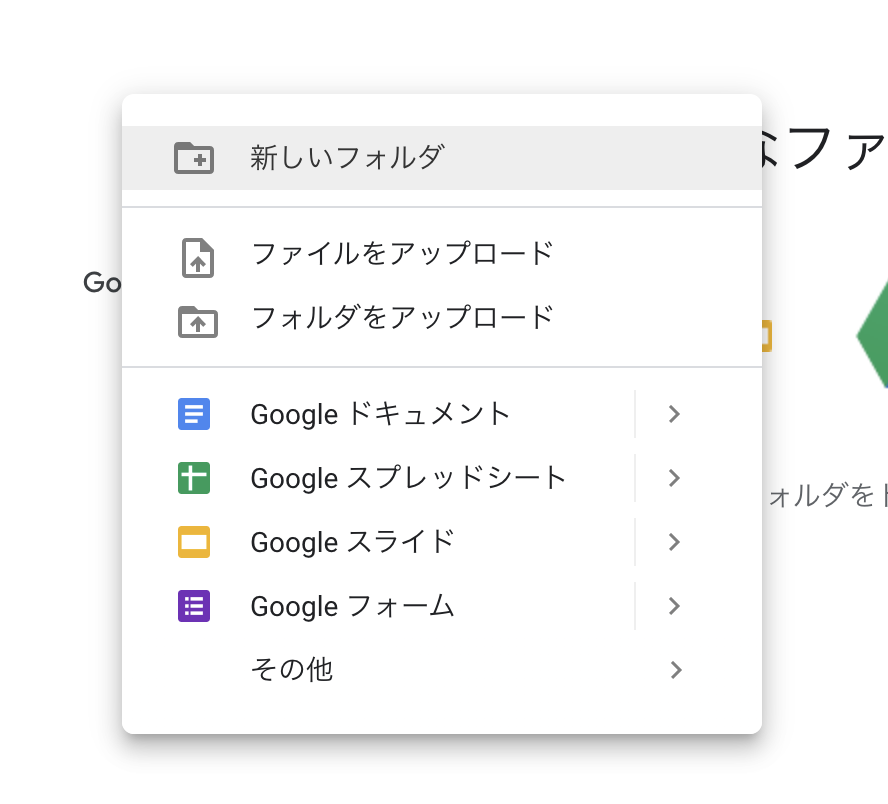
\includegraphics[scale = 0.15]{fig2-1-2.png}\caption{右クリック→新しいフォルダ。}
    \end{figure}
     
         \begin{figure}[htbp]
     \centering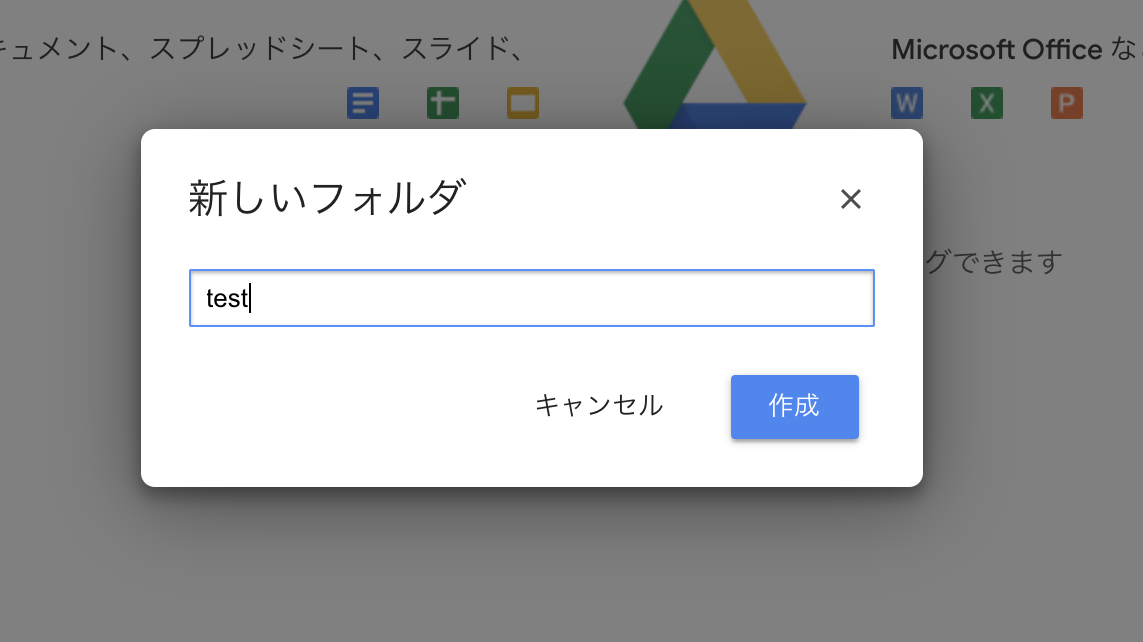
\includegraphics[scale = 0.15]{fig2-1-3.png}\caption{フォルダ名はとりあえず「test」に。}
    \end{figure}
    \\
    \item
    {\bf フォルダの中に入り、GoogleColaboratoryをインストール(有効化)。}
    
    作ったフォルダ「test」の中に入りましょう。
             \begin{figure}[htbp]
     \centering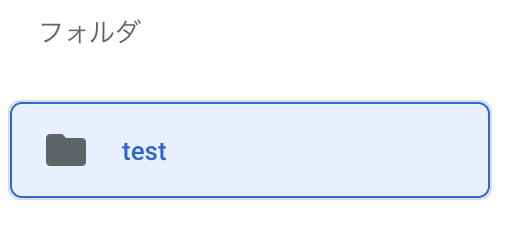
\includegraphics[scale = 0.15]{fig2-1-4.png}\caption{ダブルクリックで入れます。}
    \end{figure}
    
    そして、GoogleColaboratoryを使える状態にします。右クリック→その他→
    アプリの追加 をクリックします。
              \begin{figure}[htbp]
     \centering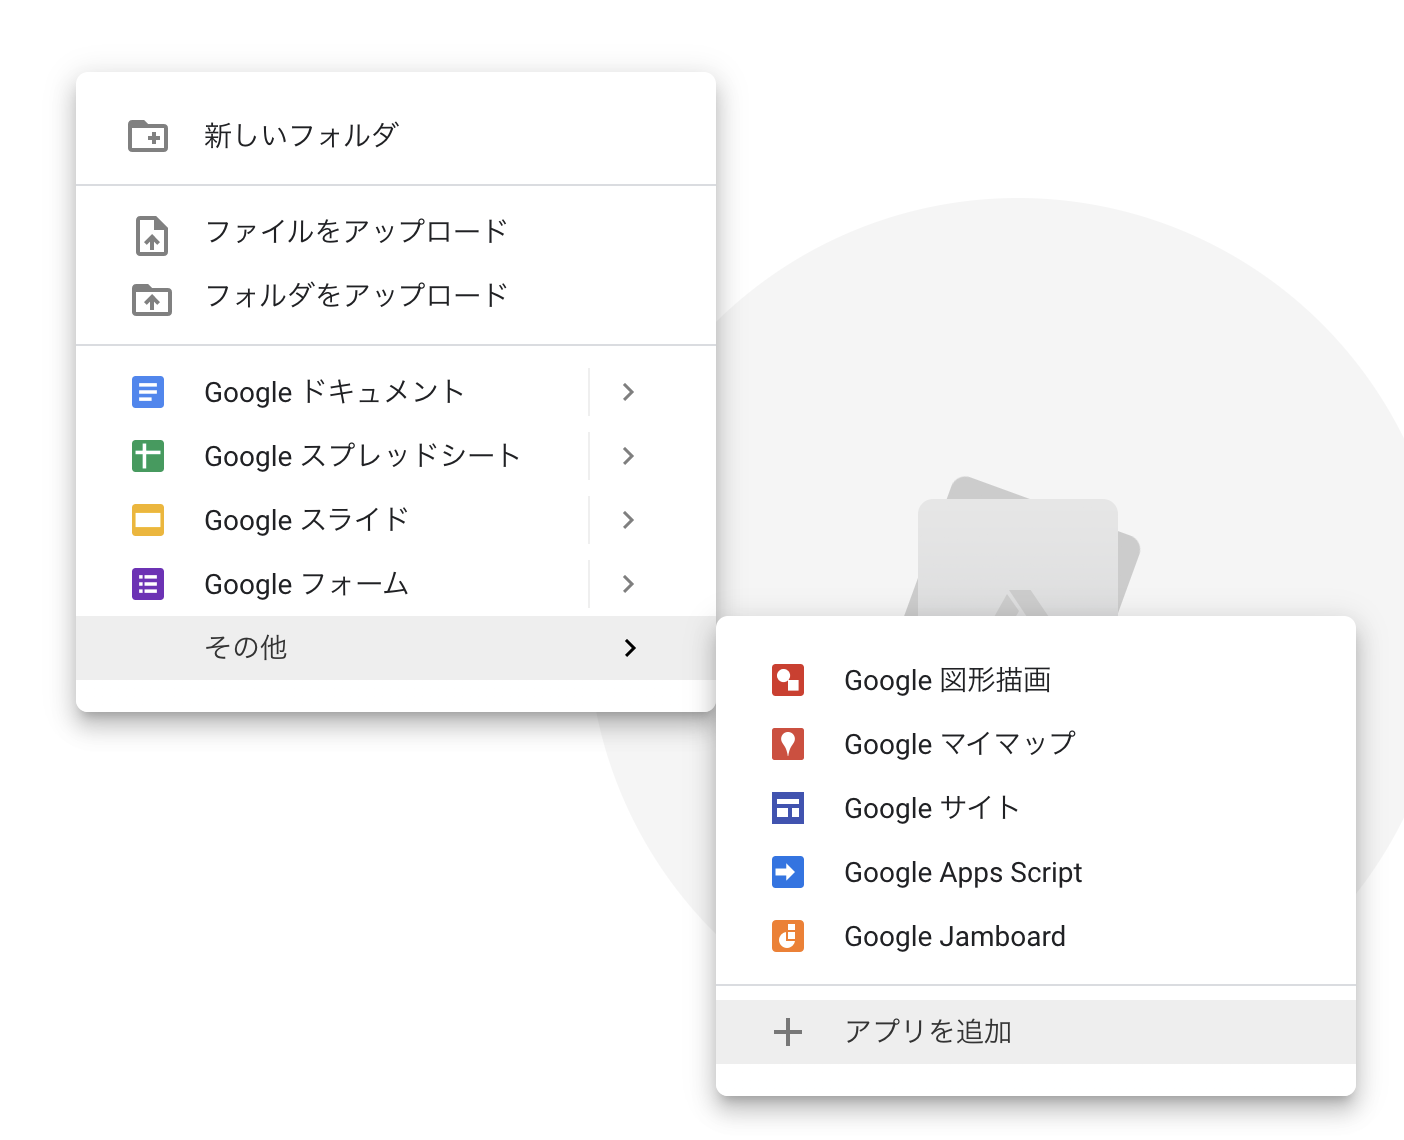
\includegraphics[scale = 0.15]{fig2-1-5.png}\caption{右クリック→その他→アプリの追加。}
    \end{figure}   
    
    「GoogleColaboratory」を探して、インストールを行います。
    
                  \begin{figure}[htbp]
     \centering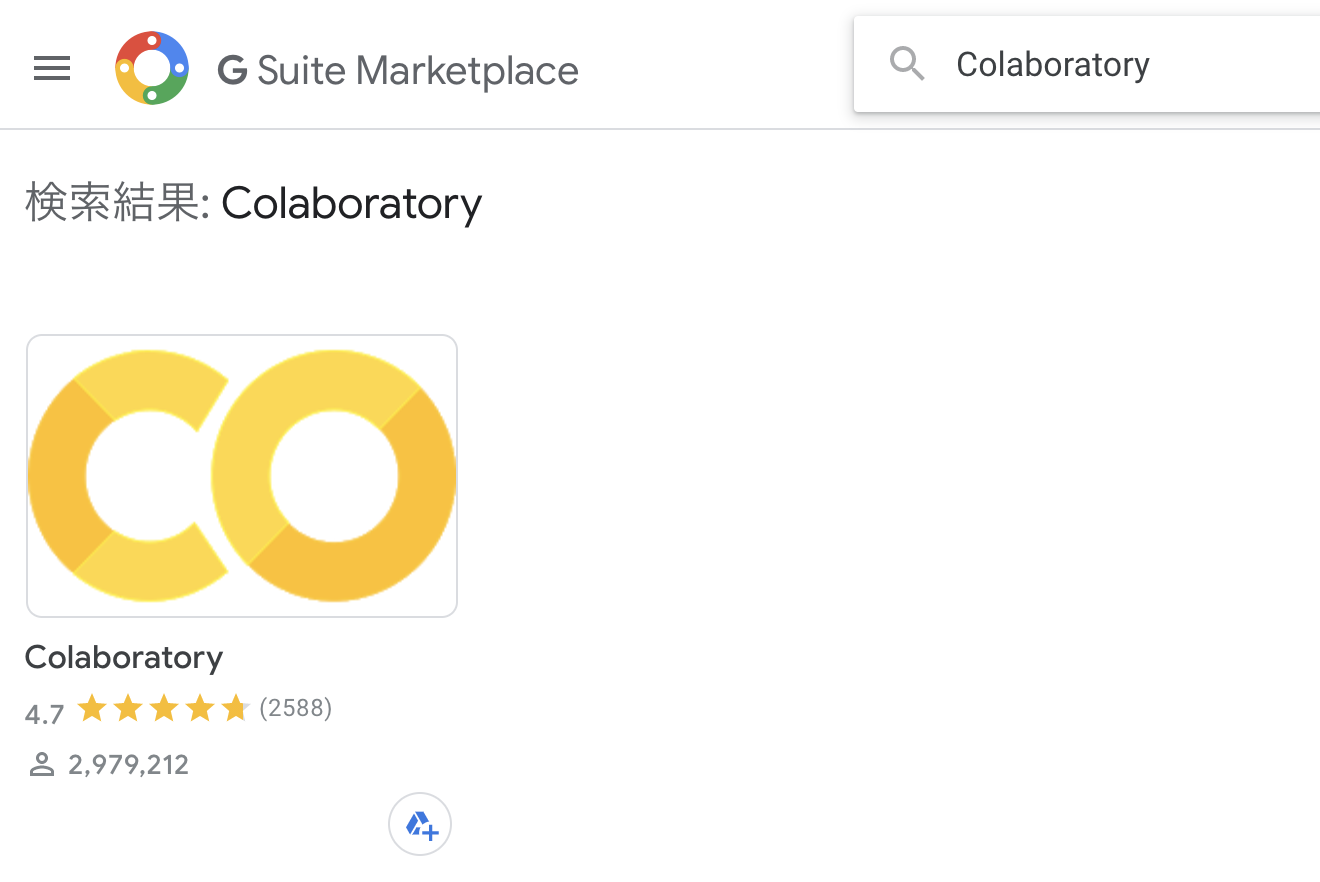
\includegraphics[scale = 0.25]{fig2-1-6.png}\caption{検索窓に「Colaboratory」と入れると出てくるはず。これをクリック。}
    \end{figure}   
    
                      \begin{figure}[htbp]
     \centering
\includegraphics[scale = 0.3]{fig2-1-7.png}\caption{インストールボタンを押すと、インストールがはじまる。}
    \end{figure}   
    
    \item
    {\bf .ipynbファイルを作成。}
    
    GoogleColaboratory上では、プログラムを.ipynb形式で扱います。.ipynbファイルを「test」フォルダの中に作ってみましょう。
    
    \begin{figure}[htbp]
     \centering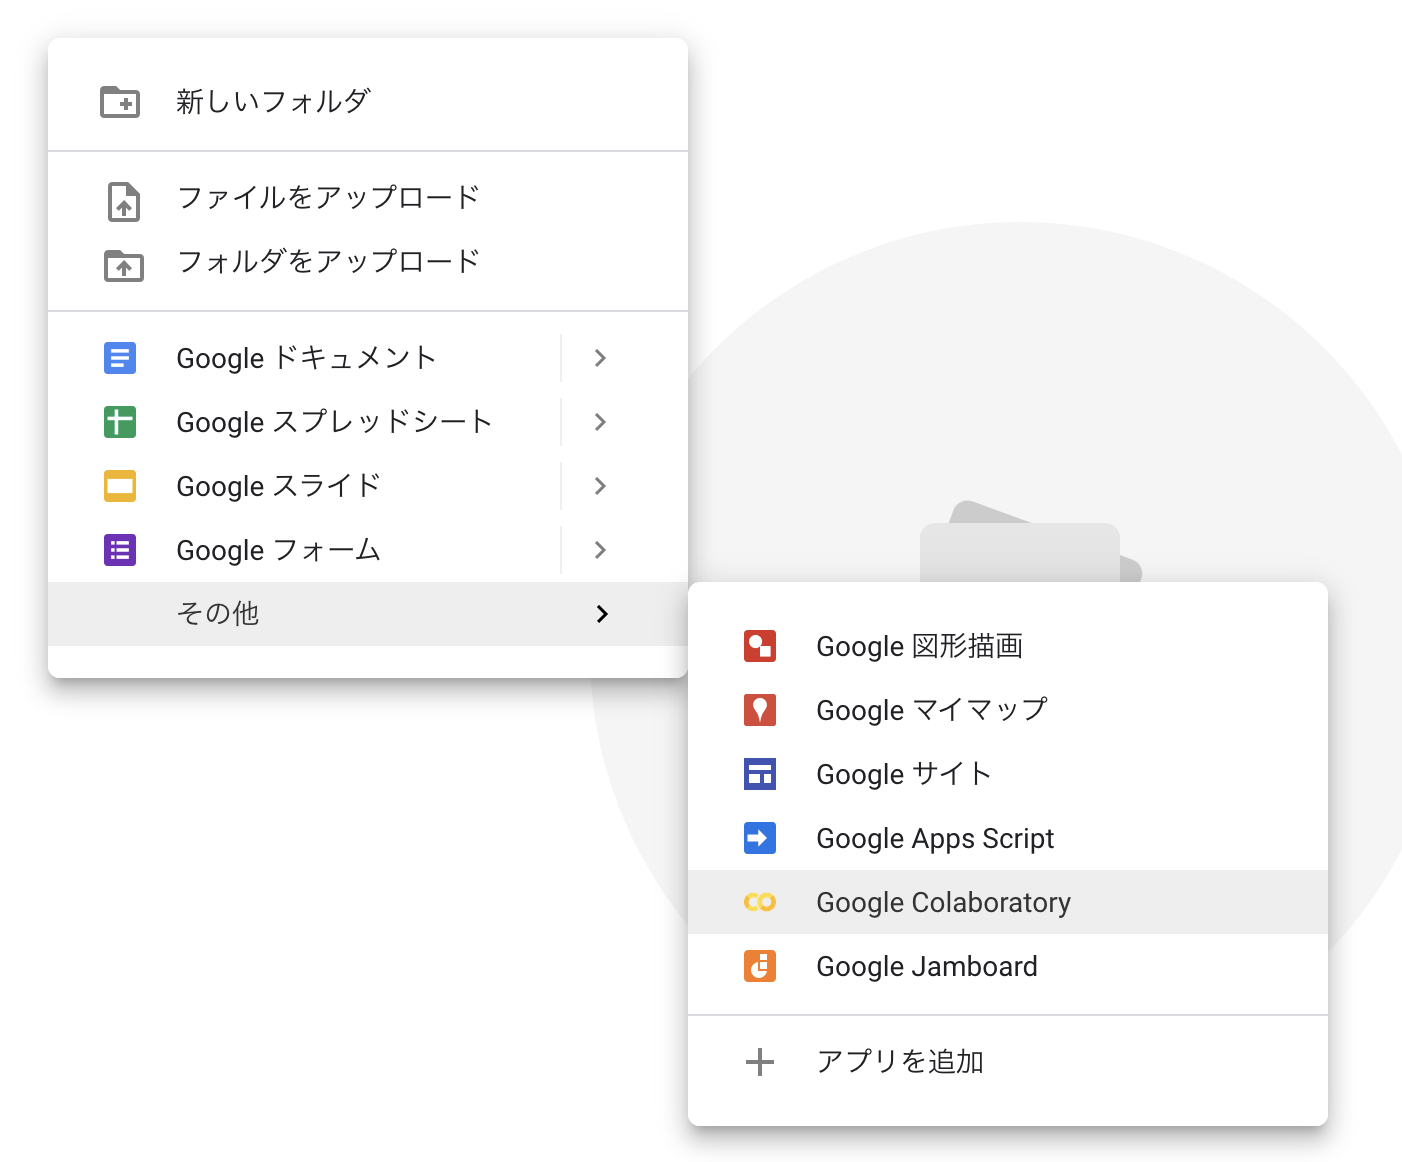
\includegraphics[scale = 0.3]{fig2-1-10.png}\caption{右クリック→「その他」に、「GoogleColaboratory」が追加されているので、クリックして.ipynbファイルを作る。}
    \end{figure}  
    \noindent
    \\
    \begin{figure}[htbp]
     \centering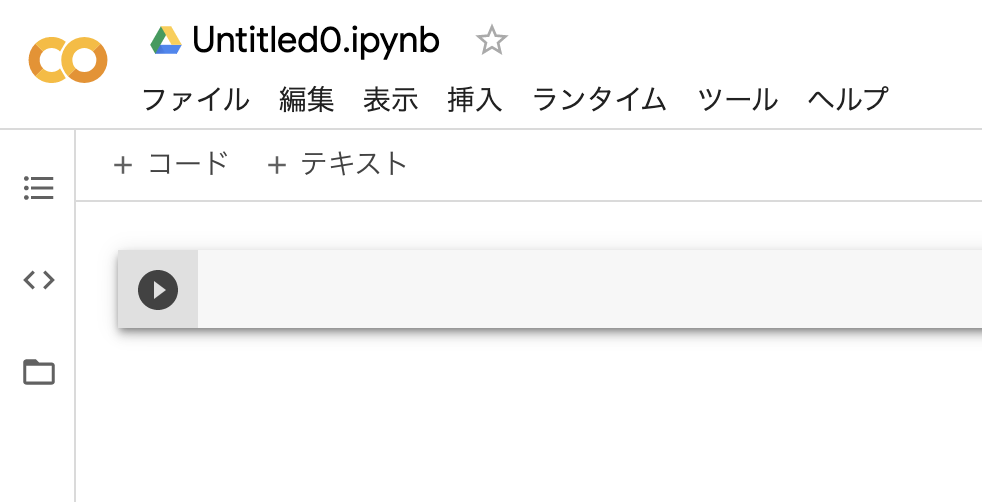
\includegraphics[scale = 0.3]{fig2-1-11.png}\caption{こんな画面が表示されれば準備完了!}
    \end{figure}     
    \noindent
    \\
    \begin{figure}[htbp]
     \centering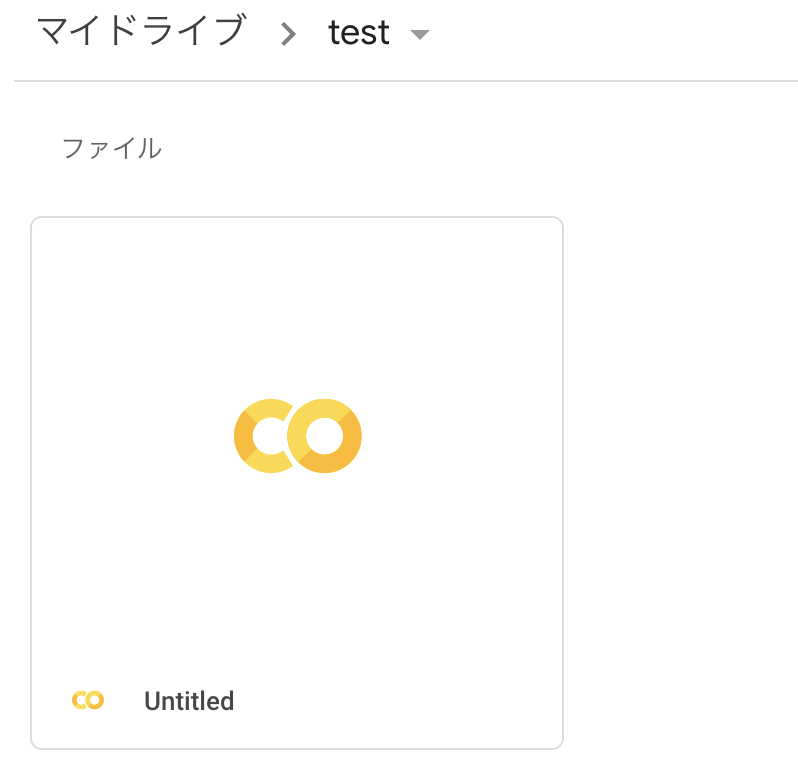
\includegraphics[scale = 0.3]{fig2-1-12.png}\caption{「test」フォルダには、ちゃんと.ipynbファイルが作成されています。}
    \end{figure}  
    \noindent
    \\
\end{enumerate}
\noindent
\\
なんと、Pythonの環境構築はこれでほぼ終了です。あとは、フォルダ内に必要に応じて.ipynbファイルを作成し、様々なプログラムを作成/実行して行きます。
\section{画面への文字表示}
いよいよPythonのプログラムを作成/実行する準備が整ったところで、簡単なプログラムを動かしてみましょう。以下のソースコード\footnote{プログラムの処理内容を記述した命令の集まりのこと。}を「一言一句違わず」「半角文字で」入力し、再生ボタンをクリック\footnote{Windowsでは「Ctrl+Enter」、Macでは「Command+Enter」を押してもOK(慣れるとこちらのほうが楽)。}して実行します。

    \begin{figure}[htbp]
     \centering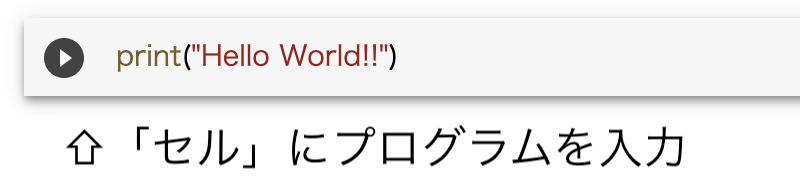
\includegraphics[scale = 0.45]{fig2-1-13.png}\caption{「セル」にプログラムを入力し、左の再生ボタンを押して実行。}
    \end{figure}
    
    以下のように「Hello World!!」と表示されれば、はじめてのPythonプログラムが動作したことになります。
        \begin{figure}[htbp]
     \centering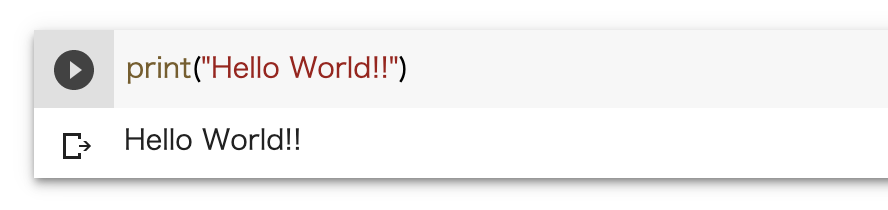
\includegraphics[scale = 0.45]{fig2-1-14.png}\caption{「Hello World!!」という文字列が表示されました。}
    \end{figure}
    
    このように、{\bf print}という命令を使うと、画面に好きな文字列を表示することができます\footnote{文字列をダブルクオーテーションで囲むのを忘れずに!あと、表示したい文字列は全角文字でもOKですが、それ以外のソースコードはすべて半角で書きましょう。}。\\
    
    \begin{itembox}[l]{\doublebox{\bf 画面に文字列を表示}}
    
    \centering \verb|print("表示したい文字列")|
    
    \end{itembox}
    \noindent
    \\[12pt]
 さて、本格的にPythonのプログラムを動かす準備が整いました。というわけで、ここからは基本的なPythonのプログラムの書き方を学んで行きましょう。Pythonは、「プログラムが非常に簡単に書ける」言語として有名で、やりたい処理を直感的に、サクサクと記述して動かすことができます。

\section{変数}

Pythonをはじめとする様々なプログラミング言語では、{\bf 変数(variable)}という「数値や文字列をしまっておく箱」に様々な値を格納しておいて、その値を必要なときに利用することによっていろいろな計算や処理を効率的に行います。先程の.ipynbファイルの新しいセルで、\verb|x|という変数を宣言\footnote{変数を新しく作ること。}し、1という値を代入\footnote{変数に値をしまうこと。}してみましょう。また、その次の行で、\verb|x|にちゃんと1が代入されていることを確認するために、\verb|print|を使って\verb|x|を表示してみましょう\footnote{変数の「中身」を表示したいときは、ダブルクオーテーションでは囲まないことに注意。}。

        \begin{figure}[htbp]
     \centering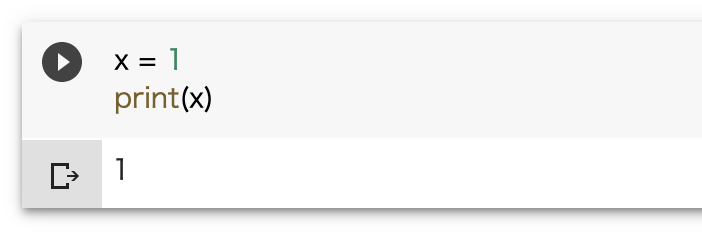
\includegraphics[scale = 0.55]{fig2-1-15.png}\caption{「1」が表示されているので、正しくxに1が代入されていることがわかります。}
    \end{figure}
    
    変数には、1のような整数だけではなく、3.14のような{\bf 実数(小数点以下がある数)}や、\verb|"こんにちは"|のような{\bf 文字列}も代入しておくことが出来ます。また、変数の名前(変数名)も自由に設定できます\footnote{「自由に」とはいっても、何でもかんでもOKというわけではなくある程度のルールがあります。とりあえず、「アルファベットの大文字小文字」と「数字」が使えて、「アンダースコア(\verb|_|)」も使える、また、「1文字目を数字で始めてはいけない」「同じ変数名を複数回使うことはできない」「Pythonですでに使われている名前(予約語)はつけられない(\verb|print|など)」というルールだけを知っておけば問題は生じないでしょう。ちなみに、一応全角文字も使えますが、使わないほうがいろいろと無難です。}。
    
            \begin{figure}[htbp]
     \centering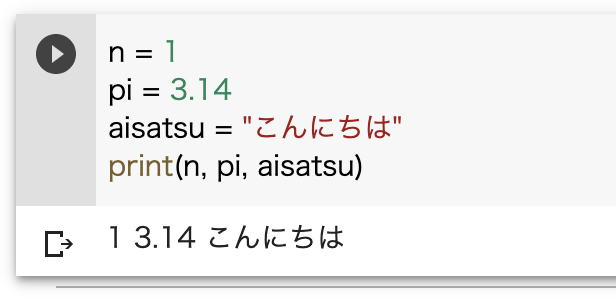
\includegraphics[scale = 0.55]{fig2-1-16.png}\caption{変数n, pi, aisatsu を宣言し、それぞれに1, 3,14, {\texttt "}こんにちは{\texttt "}を代入して表示してみました。}
    \end{figure}
複数の変数などを並べて表示するときは、このようにカンマ(\verb|,|)で区切れば表示できます。\\
    
    \begin{itembox}[l]{\doublebox{\bf 変数を宣言し、値を代入}}
    
    \centering \verb|変数名 = 代入する値|
    
    \end{itembox}
    \noindent
    \section{データ構造(リスト、タプル、集合)}
    たくさんの数値をまとめて利用したいときに、変数を1つずつ頑張ってたくさん宣言して、それぞれに値をちまちまと代入して利用するのは、なかなか手間がかかって効率が良くありません。「複数の値を一気に効率よく扱う」ためには、{\bf データ構造}を利用します。
    
    データ構造とは、複数の値(数値や文字列)を「ひとまとまりに扱う」ための方法のことをいいます。最も基本的なデータ構造は{\bf リスト}です。リストとは、複数の数値を並べてひとまとまりに宣言したものです\footnote{他の言語なんかだと、「配列」というものが現れることが多いですが、リストと配列はだいたい同じようなものです。}。以下のコードを実行してみましょう。
                \begin{figure}[htbp]
     \centering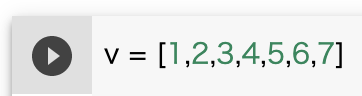
\includegraphics[scale = 0.55]{fig2-1-17.png}\caption{リストvを宣言するソースコード。}
    \end{figure}
    \noindent
    \\
    このコードでは、\verb|v|というリストに1,2,3,4,5,6,7という7つの数値を順に格納してあります。このようにリストに格納された値のことを、リストの{\bf 要素}と呼びます。リストの要素には、0番目から順に番号(インデックス)づけされており、以下のようにvの要素を読み出して利用することができます。
    
                 \begin{figure}[htbp]
     \centering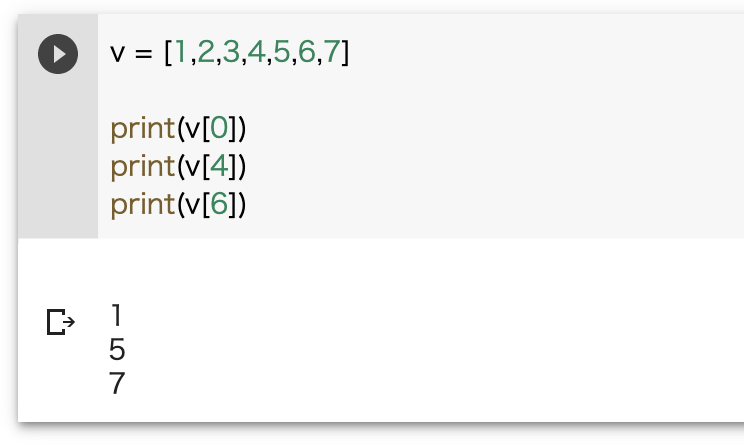
\includegraphics[scale = 0.55]{fig2-1-18.png}\caption{リストvの要素v[0], v[4],v[6]をprint文で画面に表示しています。}
    \end{figure}   
    \noindent
    \\
    リストの要素の値を上書きすることもできます。例えば、先程のvで、v[3]の値を4から100に書き換えたいときは、以下のような代入を行えばOKです。
    
                     \begin{figure}[htbp]
     \centering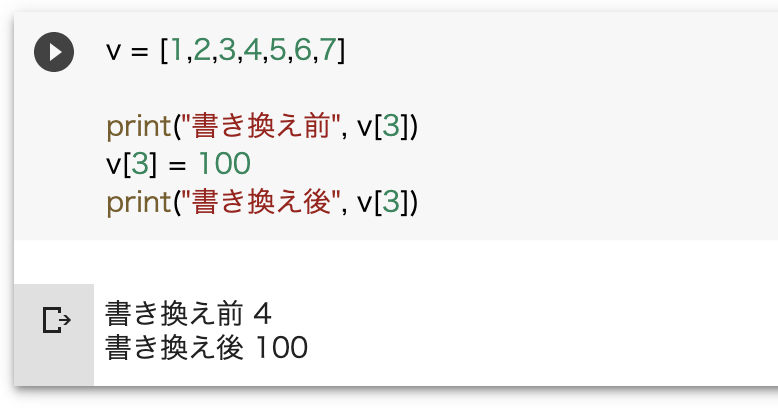
\includegraphics[scale = 0.55]{fig2-1-19.png}\caption{リストvの要素v[3]を100に書き換えました(print文で都度、値を確認しています)。}
    \end{figure}   
    \noindent
    \\
    ちなみに、リストは\verb|v=[1,2,3,4,5,6,7]|というふうに宣言をしましたが、\verb|v=(1,2,3,4,5,6,7)|というふうに宣言をした場合、{\bf タプル}というデータ構造になります。タプルはリストとほぼ同じように扱えますが、要素の書き換え(代入)ができません。
    
    次に、以下のように新しいセルで \verb|S|を宣言してみましょう。
                         \begin{figure}[htbp]
     \centering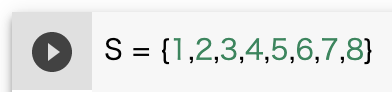
\includegraphics[scale = 0.55]{fig2-1-20.png}\caption{Sを宣言。}
    \end{figure}   
    \noindent
    \\
    このように宣言した\verb|S|を{\bf 集合(set)}と呼びます。集合とリストは何が違うのか?以下のソースコードで比較をしてみましょう。
                             \begin{figure}[htbp]
     \centering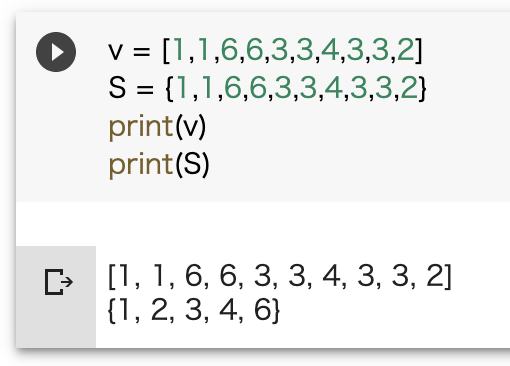
\includegraphics[scale = 0.55]{fig2-1-21.png}\caption{リストvと集合Sを比較。}
    \end{figure}   
    \noindent
    \\
    実行結果を見ると、以下の違いに気づきます。
    \begin{itemize}
    \item
    リスト\verb|v|には重複する要素が残っているのに対し、集合\verb|S|では、要素の重複が無視されている。
    \item
    リスト\verb|v|は、要素の順番が保持されているのに対し、集合\verb|S|は要素の順番が変わっている。
    \end{itemize}
    
    このように、集合というデータ構造は、要素の重複と順序を無視して数値を保持することが分かります。ですので、例えば以下のような要素の読み出しは出来ません\footnote{\verb|S|は「要素の順番」がないので、「0番目」を呼び出すことがそもそもできない。}。
    
                                 \begin{figure}[htbp]
     \centering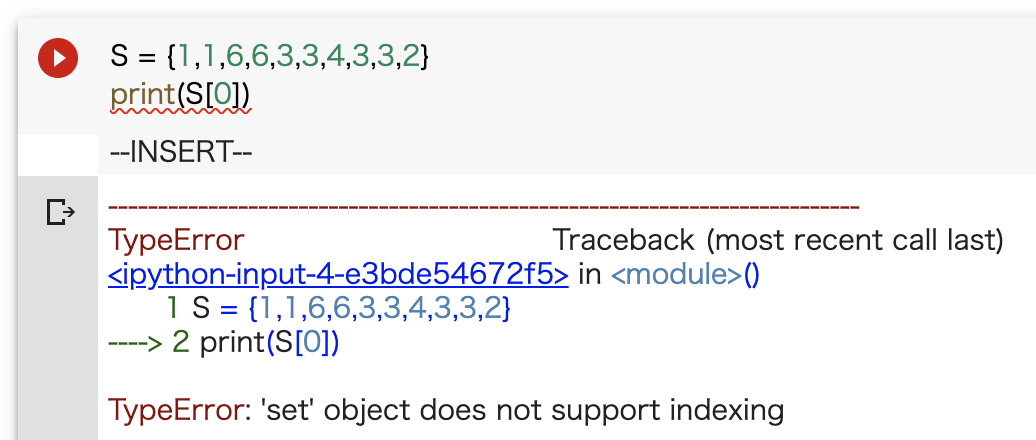
\includegraphics[scale = 0.55]{fig2-1-22.png}\caption{S[0]を読みだそうとするとエラーになる。}
    \end{figure}   
    \noindent
    \\
    
    このように、あくまで「含まれるか含まれないか」だけを問題とするデータ構造である「集合」は、高校数学で習う{\bf 集合}まさにそのものです。
    
    リスト、タプル、集合についての細かい操作(例えば、要素の追加や削除など)については、他のPython入門書に解説を譲ることとします。
\end{document}
